% !Mode\dots ``TeX:UTF-8''
% !TEX root = ../bare_jrnl.tex
\section{Introduction}
\label{sec:intro}

Before introducing the Boolean control networks, we introduce the Boolean networks at first. In 1960s, Nobel Prize winners Jacob and Monod found that ``Any cell contains a number of `regulatory' genes that act as switches and can turn one another on and off. If genes can turn one another on and off, then you can have genetic circuits.'' \cite{Jacob1961Genetic}. Inspired by these Boolean-type actions in genetic circuits, the Boolean networks (\BNs) is firstly proposed by Kauffman \cite{Kauffman1968Metabolic} for modeling nonlinear and complex biological systems. It is a type of discrete systems which based on a directed graph. In a Boolean network, each node has only two states ``0" and ``1", and each node can only be in one of these two values at a time step. The value of each node $n_i$ at the next time step is affected by the value of another node $n_j$ if there is a directed edge from $n_j$ to $n_i$, where $n_j$ and $n_i$ can be the same node. We regard these nodes as the neighboring nodes of $n_i$ and the values of these neighboring nodes is the input. And then a new value of the node $n_i$ is obtained through a series of logical operations. The logical operators used in the operation include: AND, OR, NO, XOR, and so on. Some general descriptions of the \BNs\ and their applications to biological systems can be found in \cite{Kauffman1968Metabolic}. Since then research interests in \BNs\ have been motivated by the large number of natural and artificial systems \cite{Akutsu2000Inferring, Shmulevich2002From, Faur2006Dynamical,Green2007The,Lou2010Multi}. That these systems' describing variables display only two distinct configurations, then these describing variables take only two values, i.e., $\{0,1\}$.

Then \BNs\ are naturally extended to Boolean control networks (\BCNs) when external regulation or perturbation is considered \cite{Ideker2001A}. Different from \BNs, there are three kinds of nodes in \BCNs, they are input-nodes, state-nodes and output-nodes. In \BCNs, we can only control the value of the input-nodes and observe the value of the output-nodes. However, the value of each state-node $s$ can be reflected by the value of an output-node $o$ if there exists a directed edge from $s$ to $o$. And the value of each state node $s_i$ at the next time step is affected by the value of a state-node $s_j$ (or an input-node $i$) if there is a directed edge from $s_j$ (or $i$) to $s_i$, where $s_j$ and $s_i$ can be the same node. Therefore, there are also a series of logical operations (updating rules) to obtain the new values of the state nodes and output nodes of \BCNs. \BCNs\ can be used to solve various real problems, for instance, %first \BCNs\ have been used to do 
structural and functional analysis of signaling and regulatory networks \cite{Kaufman1999A, Klamt2006A}, 
%. Second \BCNs\ have been used for 
abduction based drug target discovery \cite{Biane2017Abduction}, %. Furthermore, \BCNs\ also have been used for 
and pursuiting evasion problems in polygonal environments \cite{Thunberg2011A}. %For a better understanding, we make a brief introduction about how to use \BCNs\ to do signaling and regulatory networks' structural and functional analysis. Evolution has equipped cells with exquisite signaling systems which allow them to sense their environment. The immune system is a very important part of the signaling system, it can identify and eliminate foreign invading antigens. T-cells known as lymphocytes are a type of white blood cells, they play a central role in the immune system. T-cells can recognize protentially dangerous agents for cells and initiate an reaction against these agents. T-cells do so by T-cell receptors to detect foreign antigens bound to major histocompatibility complex molecules, and then activate, through a signaling cascade, several transcription factors. As the interaction of the antigen-specific receptor of T-cells with its antigenic ligand can lead either to cell activation (1) or to a state of profound unresponsiveness (0). There are some work  apply the \BCNs\ to study the T-cell receptor kinetics model better \cite{Kaufman1999A, Klamt2006A}. The events of T-cell receptor sianaling system can be depicted as nodes in the \BCN. Except the state-nodes, the input-nodes represent the controllable events, the output-nodes represent the events to be observed. And the updating rules of the \BCN\ represent the interation of these events. The example given in \cite{Kaufman1999A} is as follows.
 %\begin{example}The model shown in Fig.\ref{fig:6} consists of a series of events, each event requires a time step to be realized. For example, the event positive signaling is depicted as a state-node (Positive signaling, s). The input-node (Free ligand, f) of this \BCN\ is the controllable node, as we can control the event free ligand. The output-node is the node to be observed (PTK activity, k), as we would observe the event protein tyrosine kinase (PTK) activation. The positive action (influence) of the protein tyrosine kinase (PTK) activation on itself is depicted as the directed edge from the node (PTK activity, k) to itself. And the updating rule of the node (PTK activity, k)  
% \[k(t+1)=b(t)\vee (k(t)\wedge\neg s(t) )\] 
 %describes all influence to the event protein tyrosine kinase activation. The influence come from the events binding of free ligand to T cell receptors, positive signaling and protein tyrosine kinase activation itself. For more details, we refer the readers to read \cite{Kaufman1999A, Klamt2006A}. 
%\end{example}  


%By this method, we can study the properties of the 

 %\begin{figure}[thpb]
    %  \centering
      %\framebox{\parbox{3in}{
	%	\centerline{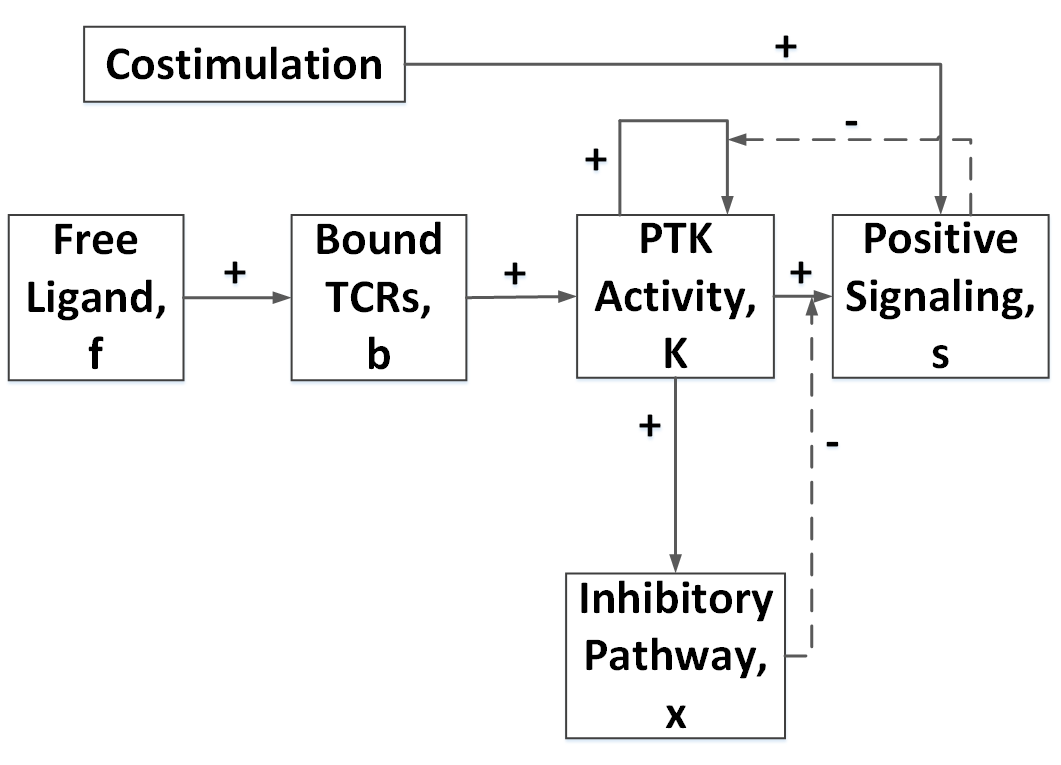
\includegraphics[scale=0.277]{figures/Fig6.png}}
	%}}
      
     % \caption{Schematic interaction diagram. f = free ligand; b = TCRs
%bound to ligand; k = receptor-associated PTK activity; x = tyrosine
%kinase-dependent inhibitory pathway; s = metabolic and mitogenic
%response. Positive and negative interactions are indicated by a plus and
%minus sign, respectively.}
  %    \label{fig:6}
  %\end{figure}

As the wide application of \BCNs, there are a lot of research work about the control-theoretic problems of \BCNs. The work in \cite{Akutsu2007Control} proves that the problem of determining the controllability of \BCNs\ is {\em NP}-hard in the number of nodes. In addition, it points out that ``One of the major goals of systems biology is to develop a control theory for complex biological systems.'' Since then, the study on control-theoretic problems in the areas of \BNs\ and \BCNs\ has drawn great attention \cite{cheng2009controllability, Zhao2010Input, Cheng2011Identification, Cheng2011Analysis,Fornasini2013Observability}. What is more, the controllability and observability are the basic control-theoretic problems of \BCNs. % Among these studies, \emph{semi-tensor product} (\STP) is one of useful tools to deal with  both \BNs\ and \BCNs\  related problems \cite{cheng2009controllability}.  We will refer to \STP\ in the {\em Section \ref{sec:pre}}. Moreover,  the concept of \BCN\'s observability was proposed firstly in \cite{cheng2009controllability}. 

However, in this paper we research the observability of the \BCNs. The concept of observability was proposed firstly in \cite{cheng2009controllability}. To date, there are four types of observability have been proposed. And they are mainly about how to get some information of the initial value of the state-nodes of the \BCNs\ by the value of their input-nodes and output-nodes. Because the value of state-nodes can be reflected by the value of output-nodes. Moreover, the value of state-nodes at the next time step is affected by the value of state-nodes and input-nodes. Such that we can control and predict the new value of the state-nodes by the value of input-nodes. Therefore, with the updating rules of \BCNs\ we get some information about the initial value of state-nodes of \BCNs\ by the value of input-nodes and output-nodes. Then based on actual application needs, different types of observability are defined to get different kinds of information about the initial value of state-nodes%Therefore, we can get some information about the initial state $s_0$ by the output of the \BCN.
%If there are multipal type of initial state $s_0$ of a \BCN\ with the same output $o_0$, then we can not determine the initial state by the initial output. 
% Then, we can use the input to control the state of \BCNs, and then get more information about the new state by the new output we observed. So that, we can get more information about the initial state of \BCN\ by controlling the input.

For convenience, we use the vectors input $i$, state $s$ and output $o$ to represent the value of the input-nodes, state-nodes and output-nodes of a \BCN\ respectively. Then an input sequence $i_0, i_1,\ldots, i_{p-1}$ consists of several inputs in sequential time steps, a state sequence $s_0, s_1,\ldots, s_{p-1}$ consists of several states in sequential time steps, and an output sequence $o_0, o_1,\ldots, o_{p-1}$ consists of several outputs in sequential time steps. Such that, for the initial state $s_0$ of a \BCN\ and its input sequence $i_0, i_1,\ldots, i_{p-1}$, we have a corresponding state sequence $s_0, s_1,\ldots, s_{p}$ and a corresponding output sequence $o_0, o_1,\ldots, o_{p}$ for this \BCN.

As we mentioned before, there are four types of observability have been proposed. The four existing observability of \BCNs\ are as follows.
%A output can be seen as a vector of the values of all output-nodes of the \BCN\ in a time step as well. Therefore a output sequence also consists of several outputs in sequential time steps. 
%Moreover,  \cite{cheng2009controllability} gives equivalent conditions for controllability of \BCNs\ and observability of controllable \BCNs. 
\begin{enumerate}
	\item The first type of observability proposed in 2009 \cite{cheng2009controllability}, and it means that every initial state $s_0$ can be determined by an input sequence $i_0, i_1,\ldots, i_{p-1}$. Such that, as we inputing $i_0, i_1,\ldots, i_{p-1}$, the corresponding output sequence ($o_0, o_1,\ldots, o_{p}$) of $s_0$ is different from the corresponding output sequence of any other types of initial state. Therefore, we can distinguish the $s_0$ from other types of initial state by this input sequence, and then we can determine whether the initial state is $s_0$ by this input sequence.
	\item 
	The second observability proposed in 2010 \cite{Zhao2010Input}, and it is determined in \cite{Li2015Controllability}. It stands that for every two distinct initial states $s_0$ and $s_0'$, there exists an input sequence $i_0, i_1,\ldots, i_{p-1}$ which can distinguish them. Such that, as we inputing $i_0, i_1,\ldots, i_{p-1}$, the corresponding output sequences ($o_0, o_1,\ldots, o_{p}$, $o_0', o_1',\ldots, o_{p}'$) of them are different from each other. Therefore, we can distinguish between these two types of initial state $s_0$ and $s_0'$ by the corresponding input sequence.	
	\item The third observability proposed in 2011 \cite{Cheng2011Identification}, and it states that there is an input sequence $i_0, i_1,\ldots, i_{p-1}$ that determines the initial state $s_0$. Such that, the corresponding output sequence of all types of initial state are different. Therefore, we can determine the initial state of the \BCN\ by this input sequence for every initial state.
	
	\item  The fourth observability proposed in 2013 \cite{Fornasini2013Observability} is essentially the observability of linear control systems, i.e., every sufficient long input sequence $i_0, i_1,\ldots, i_{p-1}$ can determine the initial state $s_0$. Such that, the corresponding output sequence of any types of initial state are different. Therefore, we can determine the initial state of the \BCN\ by every sufficient long input sequence for every initial state.
\end{enumerate}
 
%\tl{can you state the four types observability clearly and formally here?}

%\rev{****input s equence***}

In {\em Section \ref{sec:pre}}, we will present the formal definition of four observability completely and introduce their implication relationship% in the following pages. What's more, there is an approach to study large-scale \BCNs\ via network aggregations \cite{Zhang2017Observability}. In order to further improve the performance of the \BCN\ model, we make some optimizations about the definition of observability of \BCNs.     which can be checked at most once

In the four existing observability, we can not determine the initail state of \BCNs\ in real time by the first and second observability. Although we can determine the initail state of \BCNs\ in real time by the third and fourth observability, the requirements for \BCNs\ to determine the initail state are very harsh. Thus, we consider that whether we can determine the initial state of some \BCNs\ which can not be determined by the third and fourth observability.

In the porcess determining the initial state, we infer the set of possible initial states $S_k$ by observing the output of \BCN\ at every time step $k$. The input $i_k$ we chose should make every two distinct states (${s_k}^i$, ${s_k}^j$ ) in the set of possible initial states will not turn into be the same state after affected by $i_k$. And the set of possible initial states $S_{k+1}$ is derived by the input $i_k$ we chose and the new output $o_{k+1}$ we observe at the time step $k+1$, and we have $|S_{k+1}|\le|S_k|$. If $|S_{k+1}|=1$, we can determine the initial state $s_0$ of the \BCN.

While, in the third and fourth observability, at every time step $k$, we choose the same input $i_k$ no matter which output $o_k$ we observe. This makes the requirements for \BCNs\ to determine the initail state are very harsh. In order to solve this problem, we propose the concept of online observability in this paper. With the online observability, we can determine the initial state of some \BCNs\ which can not be determined before.

% With the output we observed at every time step, we can further determine the range of the initial state. As we can further determine the range, we can use different input sequence to determine the initial state. However, in the third and fourth existing observability, we have to use the same input sequence to determine the initial state without utilizing the range of the initial state. In this paper, we propose the concept of online observability which determine the initial state by making full use of the input and output of \BCNs. With the online observability, we can determine the initial state of some \BCNs\ which can not be determined before.
%we do not utilize the range of the initial state to derive the input at every time step. In the online observability, we make full use of the input and output of \BCNs\ to determine their initial state. 

In the online observability, we make full use of the input and output of \BCNs\ to determine their initial state. Therefore, a \BCN\ is online observable iff we can determine its initial state $s_0$ in real time for every initial state $s_0$. Comparing with the existing first and second observability, the online observability has the {\em real-time} property because we can determine the initial state in real time. However, comparing with the existing third and fourth observability, it has {\em interactivity} that we would make full use of the input and output of a \BCN\ to determine its initial state. With the {\em real-time} property and {\em interactivity}, we call this type of observability online observability. %In the porcess determining the initial state, we infer the set of possible initial states by observing the output of \BCN\ ar every time step. And then, we choose the input that every two distinct states in the possible initial states will not turn into be the same state after affected by this input. With the set of possible initial states, we can choose one input to refine the possible initial states set in the time step $k+1$. We repeat above procedure until the cardinality of initial states set turns into be one then we can determine the initial state of \BCNs. That is why we call this process a dynamic process. 

In order to study online observability better, we formulate the formal definition for it. Firstly, we define the derivation function to describe the derivation process of the state of \BCNs\ by their output and input at every time step. Secondly, we propose the definition of the $K$-step determinability to present that we can use a set of possible current states to determine the current state of \BCNs\ in real time in finite time steps. The derivation function and $K$-step determinability are all preparations for defining the the online observability. Thirdly, we define the online observability that for every set of possible states which derived at the time step $0$, it satisfy $K$-step determinability. By the definition, we prove that online observability is the necessary and sufficient condition of determine the initial state of \BCNs\ in real time for every initial state. Finally, we compare the online observability with existing four observability. That the online observability implies the first and second observability but not imply the third and fourth observability.

After we defined the online observability and campred it with with existing four observability, we propose two algorithms to determine it. The first one is the supertree-based algorithm, the supertree of a \BCN\ intuitively depicts how to derive the state of the \BCN\ by alternately observing the output and then deriving and deciding the input untill we can determine the state of \BCN. But there are some shortcomings in this algorithm, so we propose the algorithm based on directed graph. In the algorithm based on directed graph, we check whether the $K$-step determinability of the sets with less possible states and then check the sets with more possible states. So that, it can help us find all paths to determine the initial state of \BCNs.

Finally, in order to further illustrate the advantages of the online observability, we present how to use it to do some optimization in the process of determining the initial state. The first one is to find the shortest path and the second one is to avoid entering critical states. It because that the {\em interactivity} let the online observability has better performance than existing observability in the dynamic analysis of \BCNs.

In conclusion, in this paper we make the following contributions. 
%The four  types of observability  have many nice properties that they can be used in some useful applications. However, all of the four types of observability of \BCNs\ are offline observability which means that they can not adjust the input sequence by observing the output sequence in the process of determining the initial state of \BCNs. This property of offline observability limits the performance of \BCNs. In order to further improve the performance of \BCNs, we propose the online observability that we can determine the initial state of \BCNs\ dynamically. In other words,  the online observability decides the input sequence in each time step by observing the out sequence. In the  online observability, we infer the possible  initial states set by observe outputs of \BCN\ in the first $k$ time steps. Through the  possible  initial states, we can choose one input to refine the possible initial states set in the time step $k+1$. We repeat above procedure until the cardinality of initial states set turns into be one then we can determine the initial state of \BCNs. That is why we call this process a dynamic process. 
%In the porcess determining the initial state, we derive and decide the input in each time step by observing the out.


\subsubsection*{Contributions}
Firstly, we propose and formally define the concept of online observability of \BCNs. Comparing with existing observability, the online observability can help to determine the initial state of some biological systems. Secondly, in addition to theoretical research, we also provide two algorithms to determine the online observability for \BCNs. Finally, we present some optimization brought by the online observability of \BCNs. Including methods to find shortest path and approaches to avoid entering critical states in the process of determining the initial state of \BCNs.  These optimization further explain the advantages of online observability of \BCNs. %\rev{No important points}%\rev{***Compare with offline observabilities****} 

Then the remainder of this paper is organized as follows.
\subsubsection*{Structure}
 {\em Section \ref{sec:pre}} introduces necessary preliminaries about \BCNs, algebraic forms of \BCNs\ and the four existing types of observability of  \BCNs. {\em Section \ref{sec:online}} presents the definition of derivation function, $k$ steps determinability and online observability of \BCNs. {\em Section \ref{sec:deter}} presents how to determine the online observability of \BCNs\ by super tree and directed graph. {\em Section \ref{sec:app}} talks about some applications of the online observability of \BCNs. We also compare the online observability with offline observability in this section. {\em Section \ref{sec:con}} ends up  with the introduction of our future work.

%\tl{I will try to rewrite the intro.}

%==============================================================================================================